\section{二维离散映射系统:埃农映射}
埃农(Henon)映射是1976年由法国数学家Michel H\'{e}non提出的。Henon映射是一种可以产生混沌现象的离散映射系统。最近,用埃农映射产生的混沌序列进行图像加密的报道逐渐增多。埃农映射的迭代方程可以描述为

\begin{equation}
    \begin{cases}
        x_{n+1}=y_n+1-ax_n^2\\
        y_{n+1}=bx_n
    \end{cases}\ x,y\in [-1.5,1.5]
\end{equation}

其只有一个非线性项,埃农映射的映射过程可以分解为非线性弯曲、x方向压缩、对称变换三个子过程。其三个过程的子映射可以分别写为:
\begin{equation}
    \begin{aligned}
        T_1: & \begin{cases}
            x'=x\\
            y'=1-ax^2+y
        \end{cases}\\
        T_2: & \begin{cases}
            x''=bx'\\
            y''=y'
        \end{cases}\\
        T_3: & \begin{cases}
            x'''=y''\\
            y'''=x''
        \end{cases}
    \end{aligned}
\end{equation}

埃农映射存在两个不动点:$x^*=\dfrac{b-1\pm\sqrt{(b-1)^2+4a}}{2a},y^*=bx^*$。在经典的埃农映射中,我们通常取$a=1.4$与$b=0.3$,此时该映射出现奇怪吸引子并表现出混沌现象,在该参数下,埃农映射的吸引子和不动点如下图:
\begin{figure}
	\centering
	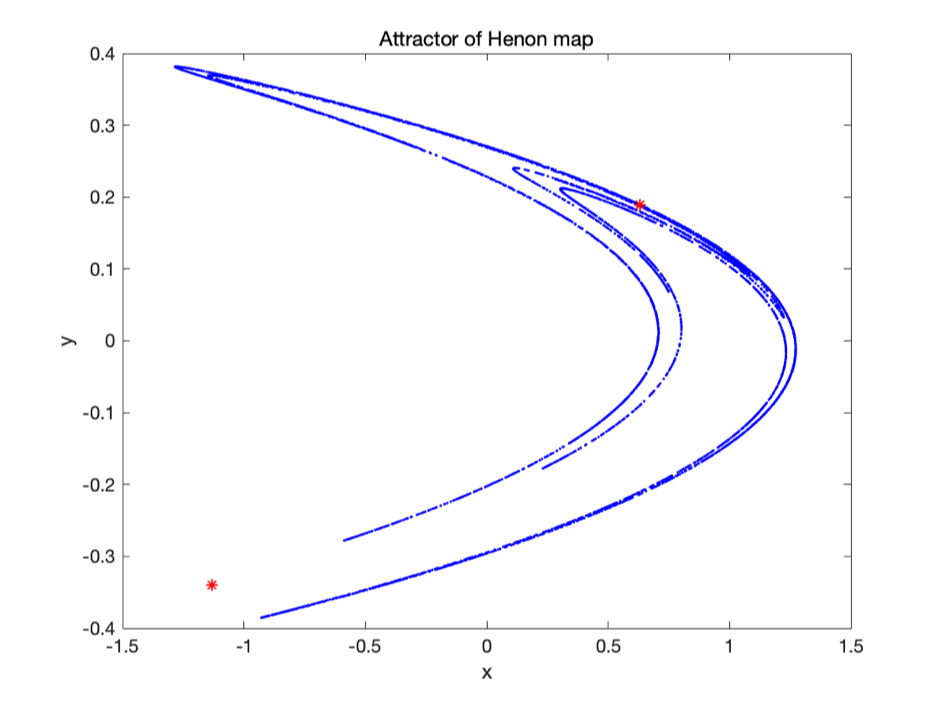
\includegraphics[scale=0.8]{henon_phase.png}
    \caption{埃农映射的吸引子和不动点($a=1.4,b=0.3$)}
    \label{fig:logi_lypn}
\end{figure}

在我们的Koopman分析中,我们在取上述参数值的情况下,通过Henon映射的迭代方程演化出一系列的数据,作为Koopman分析的源数据,以此来分析Henon映射的系统特征。

\subsection{埃农映射的动力学过程}

\subsection{埃农映射的Koopman算符本征函数}
\subsubsection{正交完备基函数空间}
\subsubsection{自然基函数空间}

\subsection{Koopman算符对埃农映射的相空间划分}
\subsubsection{埃农映射在吸引子上的划分}
\subsubsection{埃农映射的周期轨道}
\subsubsection{埃农映射的不稳定流型}

\subsection{更多的讨论}

\subsection{小结}